\chapter{Introduction}
\Atlas is a parallel flexible data-structure framework written in C++ 
and includes a Fortran 2003 object-oriented interface. \Atlas is intended 
to support a hierarchical composition of the following macro data objects.
%
\begin{itemize}
\item Grid: a list of coordinates (i.e. points) without connectivity 
rules;
\item Mesh: a collection of elements linked by precise connectivity 
rules;
\item Field: a physical quantity such as wind velocity or pressure;
\item FieldSet: a collection of Fields;
\item FunctionSpace: a given spatial discretization space (e.g. spectral, 
finite element, etc.).
\end{itemize}
%
From these objects it is possible then, for instance, to construct 
new algorithms to be tested within the context of numerical weather 
prediction (NWP), to generate and manipulate grids for production 
cases, etc. The overall structure of the library is depicted in 
Fig. \ref{fig:intro-schematics}, with the objects aforementioned 
linked together. 

We note from the figure that there is the additional object MetaData 
related to Field. MetaData is a description of a given Field (e.g. 
units, etc.).
We also note that the Mesh object is formed by the Nodes and HybridElements
objects, with the last being composed by Elements. These additional 
items represents the bricks to ultimately builds the mesh object.
 
The structure in Fig. \ref{fig:intro-schematics} will be further 
explained in chapter \ref{chap:structure}.
%
\begin{figure}[H]
  \centering
    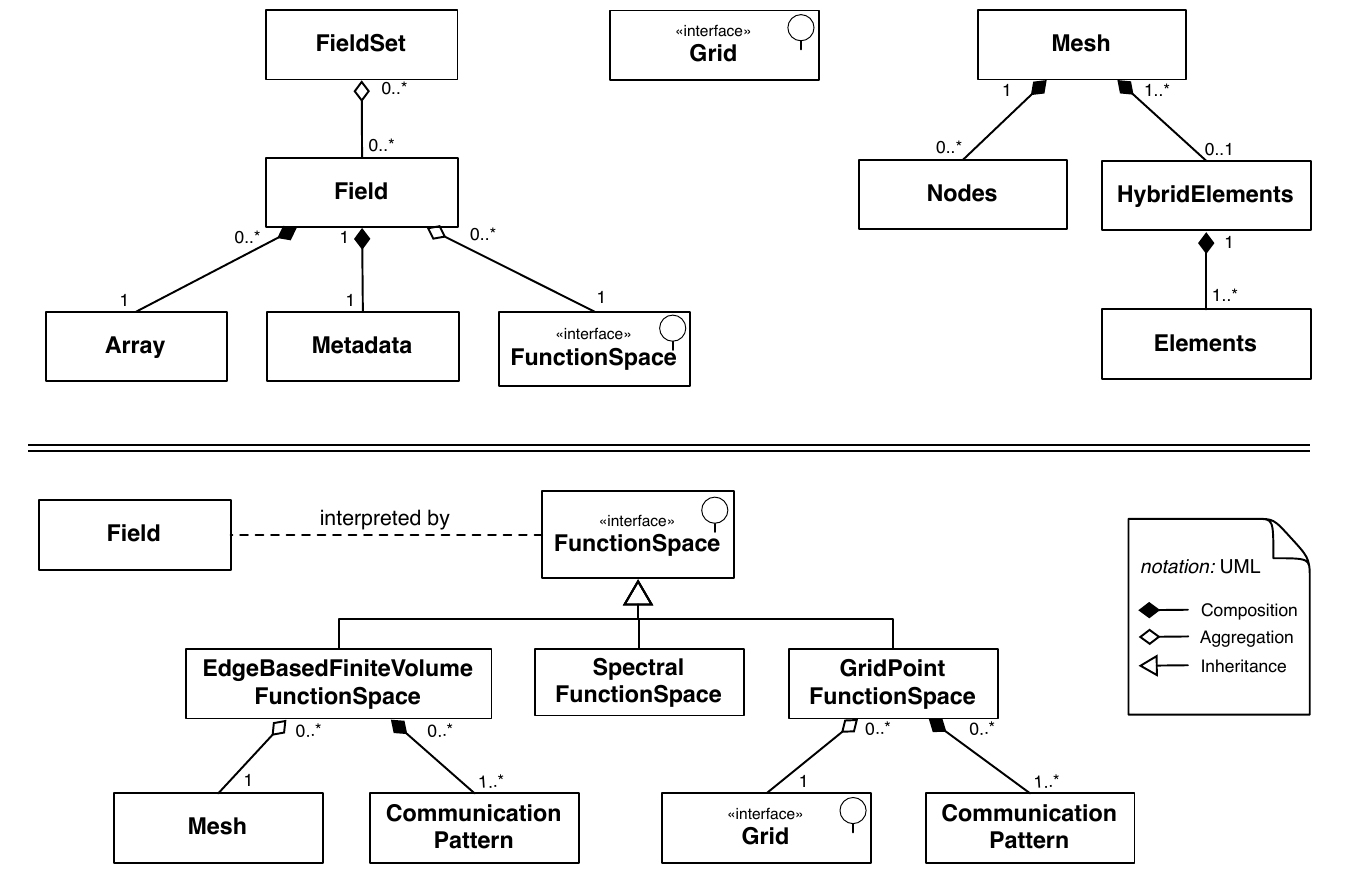
\includegraphics[width=0.95\textwidth]{imgs/schematics}
    \caption{Schematics of the \Atlas library.}
    \label{fig:intro-schematics}
\end{figure}
%